\documentclass[14pt,fleqn]{extarticle}
\usepackage[T2A,T1]{fontenc}
\usepackage[utf8]{inputenc}
\usepackage[russian]{babel}
\usepackage{amsmath}
\usepackage{graphicx}
\usepackage{tabularx}
\usepackage{boldline}
\usepackage{makecell}
\usepackage{arydshln}
\usepackage{mathtools}
\usepackage{centernot}
\usepackage{enumitem}
\usepackage{nccmath}
\usepackage{amssymb}
\usepackage[a4paper, total={6.5in, 9.5in}]{geometry}

\graphicspath{ {./images/} }
\setlength{\mathindent}{0pt}
\setlength\parindent{0pt}

\def\at{
	\left.
	\vphantom{\int}
	\right|
}


\begin{document}
	\begin{titlepage}
		
\includegraphics[scale=0.12]{logo}
		\begin{center}
			\textbf{МИНОБРНАУКИ РОССИИ}\\
			\vspace{0.2cm}
			\textbf{Федеральное государственное бюджетное образовательное учреждение высшего образования}\\
			\textbf{<<САНКТ-ПЕТЕРБУРГСКИЙ ГОСУДАРСТВЕННЫЙ ЭКОНОМИЧЕСКИЙ УНИВЕРСИТЕТ>>}\\
			\vspace{0.6cm}
			Факультет информатики и прикладной математики\\
			Кафедра прикладной математики и экономико-математических методов\\
			\vspace{1cm}
			\textbf{ОТЧЁТ}\\
			по дисциплине:\\
			\textbf{<<Модели экономической динамики>>}\\
			на тему:\\
			\textbf{<<Кластеризация экономик. Динамика экономики Японии.>>}\\
		\end{center}
		\vspace{1cm}
		Направление: 01.03.02\\
		Обучающийся: Бронников Егор Игоревич\\
		Группа: ПМ-1901\\
		\vfill
		\begin{center}
			Санкт-Петербург\\
			2022\\
		\end{center}
	\end{titlepage}
    \subsubsection*{Задание}
    
    Выполнить кластеризацию экономик, используя следующий набор показателей (отдельно за 2019, 2013 и с использованием среднего темпового показателя на временном интервале с 2013 по 2019):
    \begin{itemize}[topsep=0pt,itemsep=-1ex,partopsep=1ex,parsep=1ex]
		\item темпы роста ВВП;
		\item подушевой ВВП, темп роста ВВП;
		\item подушевой ВВП, темпы роста ВВП, темп инфляции.
	\end{itemize}

	Проанализировать полученное распределение по кластерам, миграцию между кластерами, дать содержательную интерпретацию результатов кластеризации.
	
	\subsubsection*{Решение}
	
	Данные были взяты с сайта Всемирного банка.
	
	Также если изменять параметры модели, то она всё равно будет приходить в устойчивое состояние. (Рисунок \ref{fig:M-R-W_anylogic_variance})
	\begin{figure}[h]
		\centering 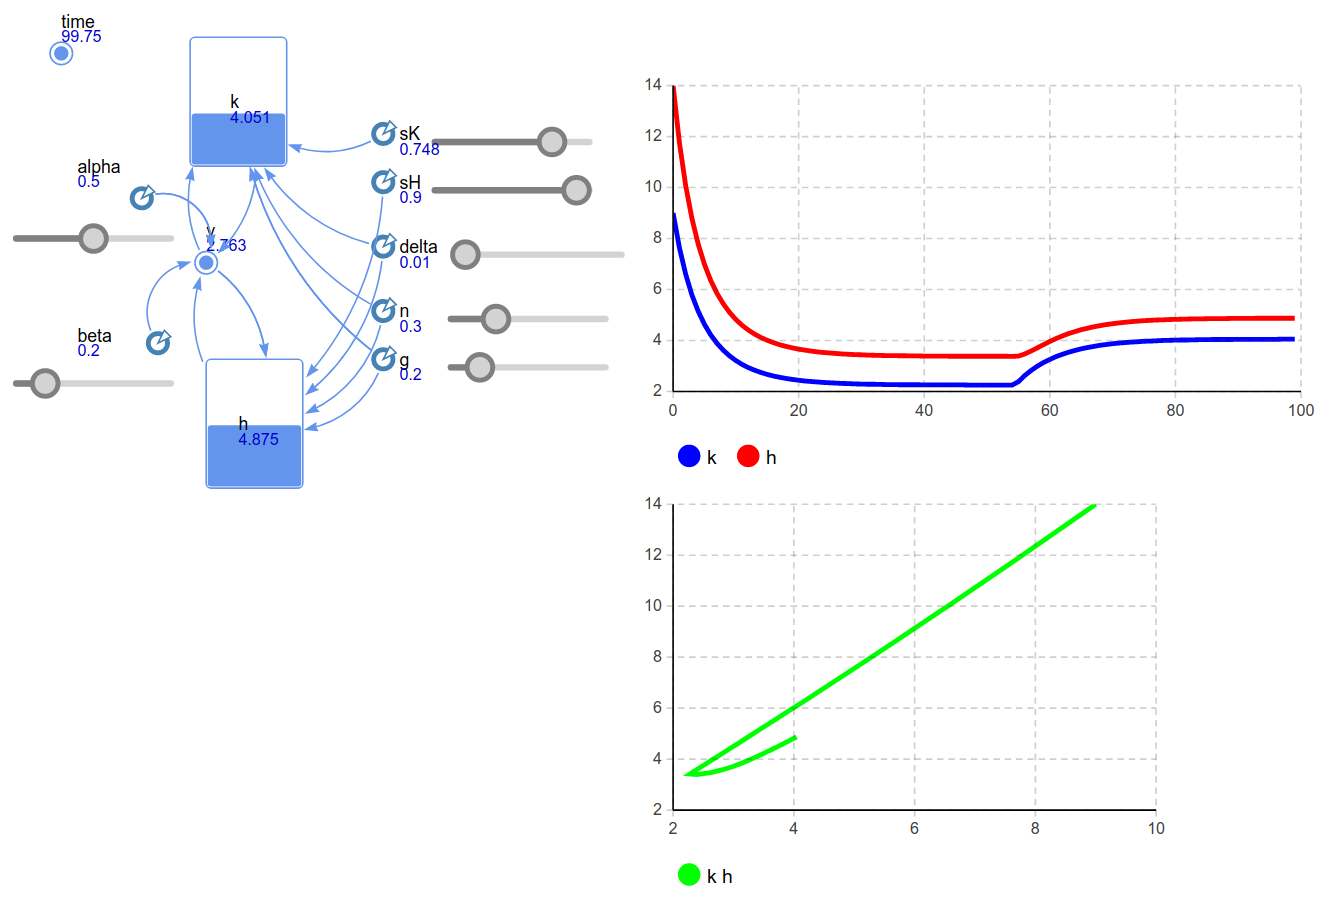
\includegraphics[scale=0.25]{M-R-W_anylogic_variance}
		\caption{Изменение параметров модели}
		\label{fig:M-R-W_anylogic_variance}
	\end{figure}
\end{document}
